\documentclass{sig-alternate-05-2015}
\usepackage{amsmath}
\usepackage[]{mcode}
\usepackage[]{algorithm2e}
\newcommand\numberthis{\addtocounter{equation}{1}\tag{\theequation}}
\lstset{numbers = left}

\begin{document}

\author{Alun Meredith\vspace{-2ex}% Toggle commenting out the command
}
\title{Options Pricing \vspace{-2ex}% to see the effect
}
\maketitle

\begin{abstract}
In this report we explore the problem of options pricing using both a closed form solution (Black-Scholes model) and  simulations (lattice model) for European and American derivatives on historic data. 
\end{abstract}

\section{Introduction}
Options are contracts to sell/buy some amount of underlying stock at a certain price at some point in the future, often used to hedge against or speculate price movements in the stock. 

Options are parametrised by the following, with only volatility not being directly observable:
\begin{itemize}
 \item $K$: Strike price
 \item $T$: Time of expiration
 \item $t$: Current time
 \item $S_t$: Stock price (at time t)
 \item $r$: Risk-free (interest) rate
 \item $c$: Value of a call option
 \item $p$: Value of a put option
 \item $\sigma$: Volatility (of stock price)
\end{itemize}

Upper limits to the individual values of the put and call options can be derived from: the value of a call option cannot exceed the stock price, the value of a put option cannot exceed the strike price, arbitrage opportunities convert these to present value of money and enforce put-call parity and ignoring tax, dividends, stock splits and transaction costs, to give\cite{book1}:

\begin{align}
p &= max(S_0 - Ke^{-rT}, 0) \\
c &= max(Ke^{-rT}-S_0, 0)
\end{align}  
 
Consider a scenario where a trader buys both a put and a call option on the same underlying stock. The profit of such a strategy is given by figure \ref{fig:Q1plot}. If the stock price increases by a large enough amount the call price becomes 'in the money' buy cheaper than market value. Equally if the price decreases enough the put option becomes 'in the money'. 

\begin{figure}
	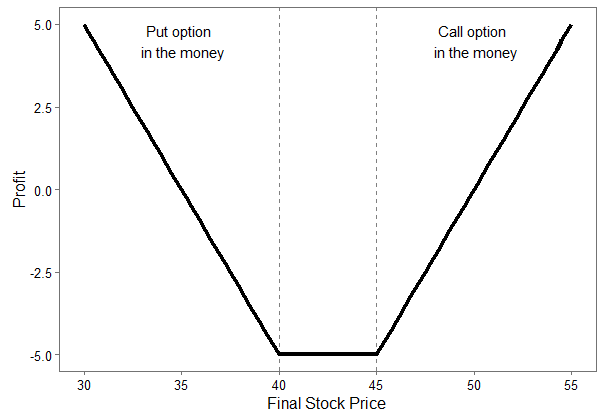
\includegraphics[width=\linewidth]{Q1plot.png}
	\centering
	\caption{Profit as a function of asset price for a combination of a call and put option on the same underlying asset with strike prices £45 and £50 respectively, assuming total option cost of £5.}
			\label{fig:Q1plot}
\end{figure} 

Although options have been used in financial markets for many years it was only in 1979 when a model for evaluating their price was published\cite{blackscholes}. The Black-Scholes equation is a closed form solution based on modelling stock movements as Brownian motion, i.e. a separable drift velocity and random walk. 

\begin{equation}
\frac{\partial c}{\partial t} + \frac{1}{2}\sigma^2S^2\frac{\partial^2c}{\partial S^2} - rc + rS\frac{\partial c}{\partial S} = 0
\label{eq:blackscholes}
\end{equation}

The data used in the following sections are put and call options written on the FTSE100 index over February:December 1994. The strike price, date, option value and underlying stock price are each recorded and the interest rate during this period is assumed to be $6.0\%$.

\section{Black-Scholes Solution}
\subsection{}
In this section we provide a solution for the call option price and through finding its derivatives prove that it satisfies the Black-Scholes equation. 

The derivative of the cumulative normal distribution is given by:
\begin{align}
N'(x) = \frac{1}{\sqrt{2\pi}}e^{-x^2/2}
\end{align}

\subsection{}

We propose that:
\begin{subequations}\label{grp1}
\begin{align}
SN'(d_1) &= Ke^{-r(T-t)}N'(d_2)\label{grp1:1}\\
d_1 &= \frac{log(S/K) + (r+\sigma^2/2)(T-t)}{\sigma\sqrt{T-t}}\label{grp1:2}\\
d_2 &= d_1 - \sigma\sqrt{T-t}\label{grp1:3}
\end{align}
\end{subequations}

To prove eq. \ref{grp1:1} evaluate the right hand side. Substituting the expression for $d_2$, factoring by $N'$ and $e^{T-t}$ before
substituting expression for $\frac{d_1}{T-t}$.

\begin{align*}\label{grp2}
RHS &= Ke^{-r(T-t)}\times \frac{1}{\sqrt{2\pi}}e^{-d_2^2/2} \\
&= Ke^{-r(T-t)}\times \frac{1}{\sqrt{2\pi}}e^{\frac{-d_1^2}{2}+d_1\sigma\sqrt{T-t}-\frac{\sigma^2}{2}(T-t)}\\
&= KN'(d_1)e^{-(\frac{\sigma^2}{2} + r)(T-t)}\times e^{d_1\sigma\sqrt{T-t}} \\
&= KN'(d_1)e^{-(\frac{\sigma^2}{2} + r)(T-t)} \times \frac{S}{K}e^{(r+\sigma^2)(T-t)} \\
 &= SN'(d_1) = LHS
\end{align*}

\subsection{}
Next calculate expressions for $\frac{\partial d_1}{\partial S}$ and $\frac{\partial d_1}{\partial S}$. They are equivalent because $\partial d_2/ \partial d_1 = 1$.

\begin{align}
\frac{\partial d_2}{\partial S} = \frac{\partial d_1}{\partial S} \frac{\partial d_2}{\partial d_1} = \frac{\partial d_1}{\partial S} = \frac{1}{SK\sigma\sqrt{T-t}}
\end{align}

\subsection{}
We show that a solution to the black-scholes equation for a call option is:
\begin{equation} \label{call_equation}
c = SN(d_1) - Ke^{-r(T-t)}N(d_2)
\end{equation}

By formulating expressions for the derivatives $\frac{\partial c}{\partial t}$, $\frac{\partial c}{\partial S}$ and $\frac{\partial^2 c}{\partial S^2}$ found in the Black-Scholes equation. 

To find $\frac{\partial c}{\partial t}$, substitute $\frac{\partial d_2}{\partial t}$, factorise by $SN'(d_1)$ (eq:\ref{grp1:1}) and cancelling terms.


\begin{align*}
\frac{\partial c}{\partial t} &= SN'(d_1)\frac{\partial d_1}{\partial t} - Ke^{-r(T-t)}N'(d_2)\frac{\partial d_2}{\partial t}\\
 &\qquad \qquad \qquad \ \ - Kre^{-r(T-t)}N(d_2) \\
\frac{\partial d_2}{\partial t} 
&= \frac{\partial d_1}{\partial t} -\frac{\sigma}{2\sqrt{T-t}} \\
\frac{\partial c}{\partial t} &= SN'(d_1)\frac{\partial d_1}{\partial t} - SN'(d_1)(\frac{\partial d_1}{\partial t} - \frac{\sigma}{2\sqrt{T-t}})\\
 &\qquad \qquad \qquad \ \ - Kre^{-r(T-t)}N(d_2) \\
\frac{\partial c}{\partial t} &= SN'(d_1)\frac{\sigma}{2\sqrt{T-t}}) - Kre^{-r(T-t)}N(d_2) \numberthis
\end{align*}

To find $N(\frac{\partial c}{\partial S})$. Compute and substitute expressions for $\partial N(d_1)/\partial S$ and $\partial N(d_2)/\partial S$. Using the (eq:\ref{grp1:1}) to cancel the second term. 
\begin{align*}
\frac{\partial c}{\partial S} &= N(d_1) +S\frac{\partial N(d_1)}{\partial t} - Ke^{-r(T-t)}\frac{\partial N(d_2)}{\partial t} \\
\frac{\partial N(d_1)}{\partial S} &= \frac{N'(d_2)}{SK\sigma\sqrt{T-t}} \\ 
\frac{\partial N(d_2)}{\partial S} &= \frac{N'(d_1)}{SK\sigma\sqrt{T-t}} \\
\frac{\partial c}{\partial S} &= N(d_1) + \frac{SN'(d_1) - Ke^{-r(T-t)}N'(d_2)}{SK\sigma\sqrt{T-t}} \\ 
\frac{\partial c}{\partial S} &= N(d_1) \numberthis
\end{align*}

\subsection{}
Finally finding an expression for $\frac{\partial^2 c}{\partial S^2}$ by finding the derivative of the previous equation. 
\begin{equation}
\frac{\partial^2 c}{\partial S^2} = \frac{N'(d_1)}{SK\sigma\sqrt{T-t}}
\end{equation}
Substituting these equations into the black-scholes formula:
Substituting $SN(d_1)$ from the definition of $c$ and removing a factor of r. 
\begin{align*}
&-rKe^{-r(T-t)}N(d_2)-\frac{SN'(d_1)\sigma}{2\sqrt{T-t}} + \frac{\sigma SN'(d_1)}{2\sqrt{T-t}} \\ & \qquad \qquad \qquad \qquad \qquad \qquad - rc + rSN(d_1) = 0 \\
LHS &= -rKe^{-r(T-t)}N(d_2) - rc + rSN(d_1)\\
&= -Ke^{-r(T-t)}N(d_2) - c + c + Ke^{-r(T-t)}N(d_2) = 0 
\\ &= RHS
\end{align*}

This shows that equation \ref{call_equation} is a solution to the black-scholes equation. In the next section we will use this solution to formulate call option prices.

\subsection{}
It can be shown that a European put option and call option have a relationship through a non arbitrage argument known as put-call parity \eqref{pc_parity} \cite{book1}. Through this we can find a closed form equation for the value of a put option:
\begin{align}
p + S_0 &= Ke^{-r(T-t)} + c \label{pc_parity}\\
p &= N(-d_2)Ke^{-r(T-t)} - N(-d_1)S \label{put_equation}
\end{align} 

\section{Black-Scholes Estimations}
In order to use the solutions to Black-Scholes \eqref{put_equation}, \eqref{call_equation} to estimate option prices and assess the validity of the model the volatility must be estimated from observed values. In the next section we discuss how much of the error is attributed to the latter of these two estimations. 

The historic estimation of volatility of a stock $\hat{\sigma}$ is given by the standard deviation of log returns over the square root of the length of the time interval in years $\tau$ \cite{book1}. The incorporation of time interval accounts for the smoothing associated with measuring over a longer interval to give an annual volatility. 

From the data ranging from $T/4 + 1$ to $T$ volatilities were estimated each day based on the previous $T/4$ window using equation \ref{volatility_equation}. Note that this is a time window rather than a number of observations window so number of observations change slightly accounting for weekends and other days the market was closed. 

\begin{align}
u_i &= ln(\frac{S_i}{S_{i-1}}) \\
\hat{\sigma} &= \frac{sd(u)}{\sqrt{\tau}} \label{volatility_equation}
\end{align}

\begin{figure}[t]
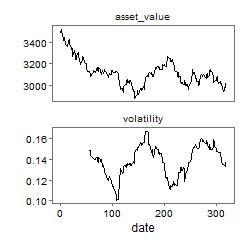
\includegraphics[width=0.8\linewidth]{../Plots/Q2_1.jpg}
\centering
\caption{Asset value and historic volatility calculated using T/4 time window for FTSE index}
\label{fig:Q2_1}
\end{figure} 

This calculation of volatility is based on the recent changes in returns of the underlying asset therefore it lags behind periods of high volatility in the asset showing peaks after turning points in the asset price. 

Comparing the estimated option price to the observed call options are systematically undervalued with this effect strongest in troughs in historic volatility(fig.\ref{fig:Q2_2}). The market appears to hold more optimism for the stock price than the past T/4 window suggests. The gradient to which absolute error in put and call option estimates change appears constant while call options appear systematically lower than put options such that the highest put option is overvalued by the estimate (fig.\ref{fig:Q2_3}). 

\begin{figure}[b]
	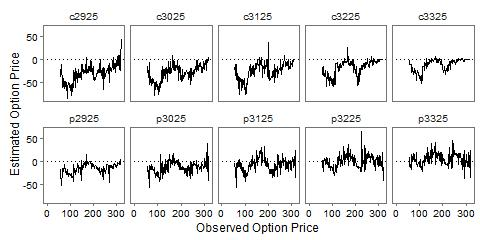
\includegraphics[width=\linewidth]{../Plots/Q2_2.jpg}
	\centering
	\caption{Observed option value vs. Estimated option value for a variety of strike prices on the FTSE index. Y = X reference line and colour/shade represents the day of measurement}
			\label{fig:Q2_2}
\end{figure}

\begin{figure}[b]
	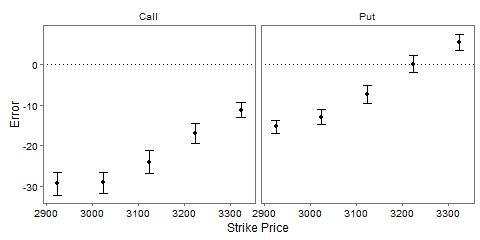
\includegraphics[width=\linewidth]{../Plots/Q2_3.jpg}
	\centering
	\caption{Change in absolute error estimating option value using Black Scholes against strike price with 95\% confidence interval}
			\label{fig:Q2_3}
\end{figure}

By plotting the change in value of $d1$ loosely interpreted as the probability the option is "in the money" shows that as the strike price moves from 2925 to 3325 the put options go from out of the money to in the money and call options vice versa. At maturity only one call option and all but one put option is in the money (Fig. \ref{fig:Q2_4}). Being "in the money" doesn't effect the direction of estimation error for put options differently from call options, this is because of the put-call parity argument and leads to the volatility smile discussed later. 

\begin{figure}[htbp]
	
\includegraphics[width=\linewidth]{../Plots/Q2_4.jpg}
	\centering
	\caption{Change in the value of d1, loosely interpreted as probability of option being "in the money", over time for each option.}
			\label{fig:Q2_4}
\end{figure}

\section{Implied Volatility}
As shown by the systematic differences between estimation and observed values in option prices the model being used is not a reflection of market activity. In this section we explore the idea that the estimation of volatility is at fault. 

Historic volatility is limited by its ability to only look at the past action of the underlying asset whereas traders act more predictively trying to assess how the market will react to upcoming events. By keeping the underlying assumptions of the Black-Scholes model the volatility estimated by the market can be computed, as it is the only parameter of the Black-Scholes model not directly observable.   

This measure is known as 'Implied Volatility'. To find this a bisection method is used (where error is the difference between computed and observed option values): 

\begin{algorithm}
 Choose interval such that: $I_l < \hat{\sigma} < I_u$\; 
 \While{ $Error \nsim 0$ }{
   $mid = (I_l + I_u) / 2$\;
  \eIf{$Error(mid) > 0$}{
   $I_l = mid$\;
   }{
   $I_u = mid$\;
 }
 }
 \KwRet{mid}
 
 \caption{Finding implied volatility $\hat{\sigma}$ through bisection method}
\end{algorithm}

\begin{figure}[ht]
	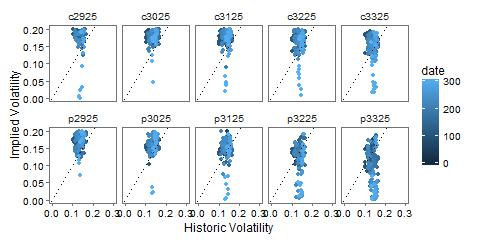
\includegraphics[width=\linewidth]{../Plots/Q3_1.jpg}
	\centering
	\caption{Implied Vs. Historic volatility for each option}
			\label{fig:Q3_1}
\end{figure}

Historic volatility is generally smaller than implied volatility for this asset. Implied volatility also has generally larger variance especially towards the date of maturity where implied volatility decreases significantly. As the strike price increases the variance in implied volatility also increases and average decreases (fig.\ref{fig:Q3_1}). 

\begin{figure}[h]
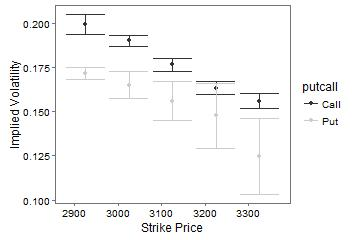
\includegraphics[width=0.8\linewidth]{../Plots/Q3_2.jpg}
\centering
\caption{Implied volatility vs. strike price for put and call options with interval of 2 standard errors (~95\% confidence)}
\label{fig:Q3_2}
\end{figure} 

Figure \ref{fig:Q3_1} shows that strike price has an impact on implied volatility, this is counter intuitive because volatility is a measure of the underlying asset and only through approximating it through Black-Scholes and option values does a relationship occur. This is known as the volatility smile. 

In figure \ref{fig:Q3_2} we see the relationship between implied volatility and strike price more clearly. Here it decreases as strike price increases. Uses the no arbitrage opportunities argument it can be shown that implied volatility for put and call options should be the same \cite{book1}. This assumption may be flawed given that implied volatilities for the test data are similar but generally do not overlap within a 95\% confidence interval. 

\section{American Options}
Until now we have only discussed European options, in practice however American style options are more common. The primary difference between the two is the exercise right. That is American options can be exercised at any time whereas European options may only be exercised at the date of maturity. 

American options are always worth at least the same amount as European options and often more. The fact that they are always worth at least the same amount is trivial since they give the option owner as much rights as the European option and more. Therefore at its worst an American option can be exercised at the date of maturity for the same value as a European option of the same strike price. 

American put options are exercised early when they are sufficiently in the money. This is because they have a significant upper boundary on how much they are worth. As an extreme example when the asset value is approximately zero the value of the option cannot increase and therefore should be exercised early where the earnings can increase at the risk-free rate. 

Why an American call option is often worth more than a European one is less obvious, this is because there is no inherent advantage to exercising an option early. Consider a trader half way through the life of an option considering exercising their option for a profit. If he does so and the stock price increases still then the trader would still have been able to buy that stock at maturity and gained interest on his money while waiting. If the stock price decreases then the value of the trader's stock he has just bought decreases in parallel to the option he would otherwise have had. If it decreases below the strike price then the trader has lost money whereas the option is protected against this (beyond the initial cost of the option). 

However the difference in value of an American and European option is inherently based on the likelihood $\times$ value of exercising that option early. Therefore  there are some instances where these options are exercised early. Primarily this is due to dividends, when a dividend is issued on a stock the value decreases. Alternatively a trader could strongly believe the underlying stock is at the turning point of a peak/trough. In both of these cases the Brownian motion assumption is broken and changes in asset value are predicted. If these changes are greater than the interest (time value) gained but not exercising early then it is wise to do so.

An argument against this is that the options themselves can be traded, therefore it should not matter that you cannot exercise a European option early. However this assumes a liquid market. It is unlikely someone will buy your European option for the same value the day before a dividend. 

\section{Binomial Lattice Model}
An alternative way of estimating call and put option prices is through the Binomial lattice model. This models the underlying asset as a set of n nodes time $\delta t$ apart. At each of these nodes there is a probability $p$ the asset will increase in price by factor $u$ and probability $1 - p$ that it will decrease by factor $d$. 

This produces a lattice of asset value and probabilities for each time step. At maturity the value of the option for each asset value is known, backward propagating this through the probability distribution of the lattice gives the value of the option at the current time. I.e. each parent node has asset value equal to weighted average of the child nodes. 

The parameters of this model can be estimated analytically by constructing a risk-free portfolio of shares and options in the underlying asset and applying a no-arbitrage assumption \cite{book1}.

\begin{subequations}\label{grp4}
\begin{align}
u &= exp(\sigma\sqrt{\delta t}) \\
d &= exp(-\sigma\sqrt{\delta t}) \\
p &= \frac{exp(r\delta t) - d}{u - d}
\end{align}
\end{subequations}

A large number of options are simulated in a process similar to bootstrapping. 1 option is sampled from the test data as a base and  it's volatility varied by sampling the volatilities in the test data 10,000 times with replacement. The Black Scholes and Binomial methods described above are used to estimate option prices. 

\begin{figure}[h]
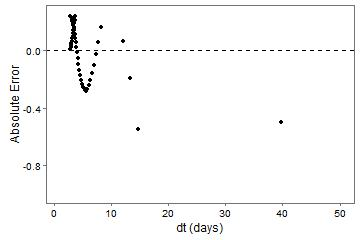
\includegraphics[width=0.8\linewidth]{../Plots/Q5_1.jpg}
\centering
\caption{Absolute error in binomial vs Black-Scholes estimation of option value for 10,000 simulated options with differing volatilities. 95\% confidence interval.}
\label{fig:Q5_1}
\end{figure} 

As the time step decreases the difference in binomial and black scholes approximations approaches 0. This observation is also seen on the test data by estimating the call prices of options using a binomial lattice for 4 different time steps and comparing to the previous Black-Scholes estimates \ref{fig:Q5_2}. As before the difference approaches 0 and variance reduces as time step decreases. 

\begin{figure}[h]
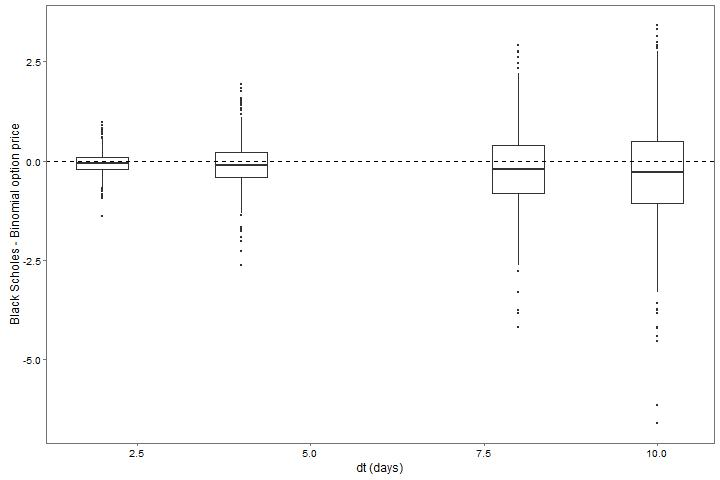
\includegraphics[width=0.8\linewidth]{../Plots/Q5_2.jpg}
\centering
\caption{Absolute error in binomial vs Black-Scholes estimation of option value for test data}
\label{fig:Q5_2}
\end{figure} 

\section{American Binomial Lattice}
American options are algorithmically computed in a very similar manner to European ones with the exception that at each node in the lattice the current value of the option must be considered in addition to the value propagated backwards from maturity. 

\begin{lstlisting} 
[...]
for tau=1:N
	for i= (tau+1):2:(2*N+1-tau)
		hold = p_u * PVals(i+1) + p_d * PVals(i-1);
		PVals(i) = max(hold, K-SVals(i));
	end
end
\end{lstlisting} 

In the above algorithm the asset price for each node of the lattice $SVals$ and option value at maturity of each of the possible mature asset values $KVals(i = 1:2:2*N+1)$ have already been computed.

Line one loops through each layer of the lattice (from maturity to present day), while line 2 loops through each node at that time step. Line 3 computes the expected return from this node $hold$ as the weighted value of the child nodes, which for i = 1 are the mature nodes otherwise, including accounting for risk free rate of exercising put option early. Line 5 computes which is greater, the current value at that node $K - SVals(i)$ (value of exercising early) or the expected return. These values are then used to compute the values for the previous time-step until present day.   

Evaluating American put option prices for the test data and comparing the difference between European option price shows very small potential improvements in value, always $\geq 0$ and increasing for larger strike prices. This supports the arguments made in section 5 that American options are always at least at valuable as European ones and as the put option becomes more in the money the benefit to exercising early increases. Therefore the points where the values diverge the most correspond to troughs in the asset price (around day 150 and 230), where it is best to exercise early considering the data available. 

\begin{figure}[h]
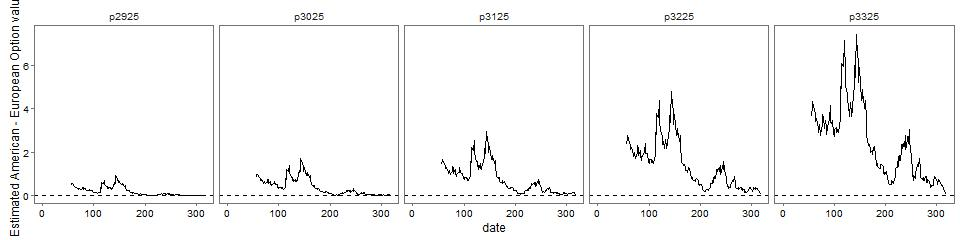
\includegraphics[width=\linewidth]{../Plots/Q6_1.jpg}
\centering
\caption{Absolute difference in American vs. European option value for test data}
\label{fig:Q6_1}
\end{figure} 

\section{Conclusion}
There are two main ways of estimating option values through a Brownian motion model of stock. The Black-Scholes Equation and the binomial lattice model. The binomial lattice model approximates the Black-Scholes as dt goes to 0. 

Both methods require volatility to be estimated and as volatility is the only parameter of the Black-Scholes equation which cannot be directly observed it's market value can be implied. 

American style options which can be exercised early are always at least as valuable as their European equivalent due to increased flexibility, however call options on non-dividend paying stock should not be exercised early outside exceptional circumstances whereas put options should be exercised early when sufficiently in the money. 

We have evaluated these factors on a historic FTSE100 index to show they hold for this historic data. 

\bibliographystyle{abbrv}
\bibliography{sigproc}  % sigproc.bib is the name of the 
\end{document}